\let\lesson\undefined
\newcommand{\lesson}{\phantomlesson{Bài 1: Sự chuyển thể}}
\chapter[Mô hình động học phân tử và sự chuyển thể của các chất]{Mô hình động học phân tử và sự chuyển thể của các chất}
\section{Lý thuyết}
\subsection{Mô hình động học phân tử về cấu tạo chất}
Mô hình động học phân tử về cấu tạo chất có những nội dung cơ bản sau:
\begin{enumerate}[label=\arabic*.]
	\item Các chất được cấu tạo từ các hạt riêng biệt gọi là phân tử.
	\item Các phân tử chuyển động hỗn loạn, không ngừng. Nhiệt độ của vật càng cao thì tốc độ chuyển động của các phân tử cấu tạo nên vật càng lớn.
	\item Giữa các phân tử có lực hút và đẩy gọi chung là lực liên kết phân tử.
\end{enumerate}
\subsection{Cấu trúc của chất rắn, lỏng, khí}
\subsubsection{Phân biệt cấu trúc của chất rắn, lỏng, khí}
\begin{center}
	\begin{tabular}{|p{3cm}|p{3cm}|p{3cm}|p{3cm}|}
		\hline
		\rowcolor{red!25!white}
		\thead{Đặc điểm}&\thead{Thể rắn} &\thead{Thể lỏng}&\thead{Thể khí}\\
		\hline
		Khoảng cách giữa các phân tử & Rất gần nhau (cỡ kích thước phân tử) & Xa nhau & Rất xa nhau (gấp hàng chục lần kích thước phân tử)\\
		\hline
		Lực tương tác phân tử & Rất mạnh & Nhỏ hơn trong chất rắn & Rất yếu\\
		\hline
		Sự sắp xếp của các phân tử & Trật tự & Kém trật tự hơn & Không có trật tự\\
		\hline
		Chuyển động của các phân tử & Chỉ dao động quanh vị trí cân bằng cố định & Dao động quanh vị trí cân bằng luôn luôn thay đổi & Chuyển động hỗn loạn \\
		\hline
		Hình dạng & Hình dạng riêng xác định & Có hình dạng của bình chứa & Có hình dạng của bính chứa\\
		\hline
		Thể tích & Xác định & Xác định & Chiếm toàn bộ thể tích bình chứa\\
		\hline
	\end{tabular}
\end{center}
\subsubsection{Chất rắn kết tinh và chất rắn vô định hình}
\begin{itemize}
	\item \textbf{Chất rắn kết tinh} là chất mà các hạt (phân tử, nguyên tử, ion) cấu tạo nên nó ở thể rắn, liên kết với nhau một cách chặt chẽ, sắp xếp theo một trật tự hình học xác định tạo thành các mạng tinh thể.\\
	\textit{\textbf{Ví dụ:}} muối ăn, thạch anh, kim cương, nước đá, \dots
	\begin{center}
		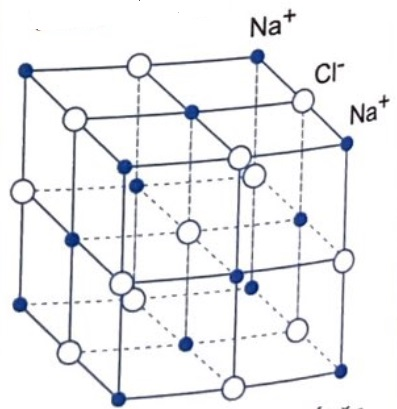
\includegraphics[width=0.2\linewidth]{../figs/VN12-Y24-PH-SYL-001-3}
		\captionof{figure}{Cấu trúc tinh thể muối ăn.}
	\end{center}
	\item \textbf{Chất rắn vô định hình} là chất ở thể rắn mà các hạt tạo nên nó không tạo thành mạng tinh thể.\\
	\textbf{\textit{Ví dụ:}} thuỷ tinh, nhựa đường, sôcôla, \dots
\end{itemize}
\subsection{Sự chuyển thể}
Khi các điều kiện như nhiệt độ, áp suất thay đổi, chất có thể chuyển từ thể này sang thể khác.
\begin{itemize}
	\item Quá trình chuyển từ thể rắn sang thể lỏng của các chất được gọi là \textit{sự nóng chảy}. Quá trình ngược lại gọi là sự đông đặc.
	\item Quá trình chuyển từ thể lỏng sang thể khí (hơi) của các chất được gọi là \textit{sự hoá hơi}. Quá trình chuyển ngược lại gọi là sự ngưng tụ.
	\item Trong một số điều kiện, chất rắn có thể chuyển sang thể khí (hơi). Quá trình này gọi là sự thăng hoa. Quá trình ngược lại gọi là sự ngưng kết.\\
	\textbf{Ví dụ:} Sự thăng hoa dễ dàng của băng phiến ở nhiệt độ thường. Sự ngưng kết của hơi nước trong không khí tạo thành sương muối.
	\begin{center}
		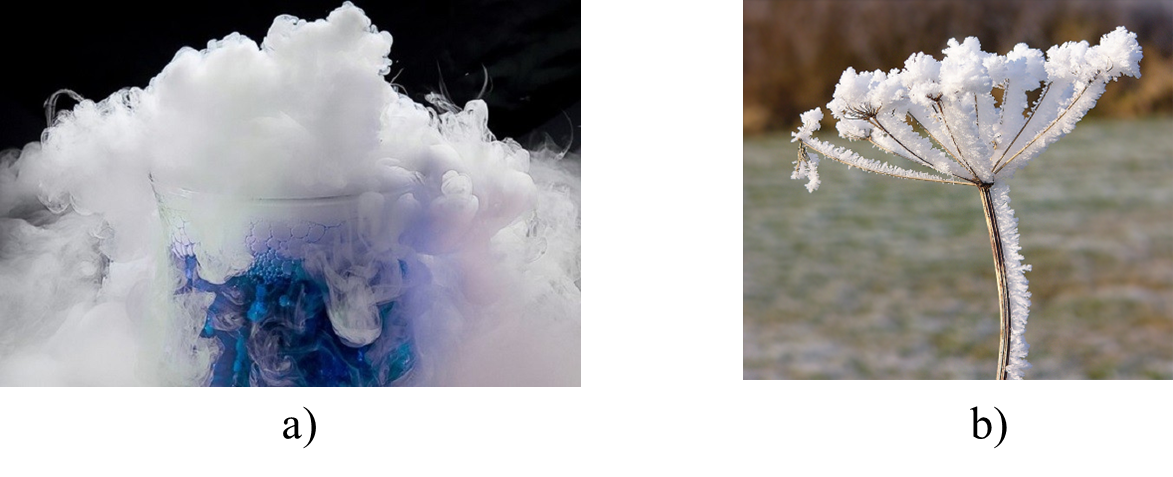
\includegraphics[width=0.7\linewidth]{../figs/VN12-Y24-PH-SYL-001-7}
		\captionof{figure}{a) Đá khô thăng hoa; b) Sương muối.}
	\end{center}
\end{itemize}
\begin{center}
	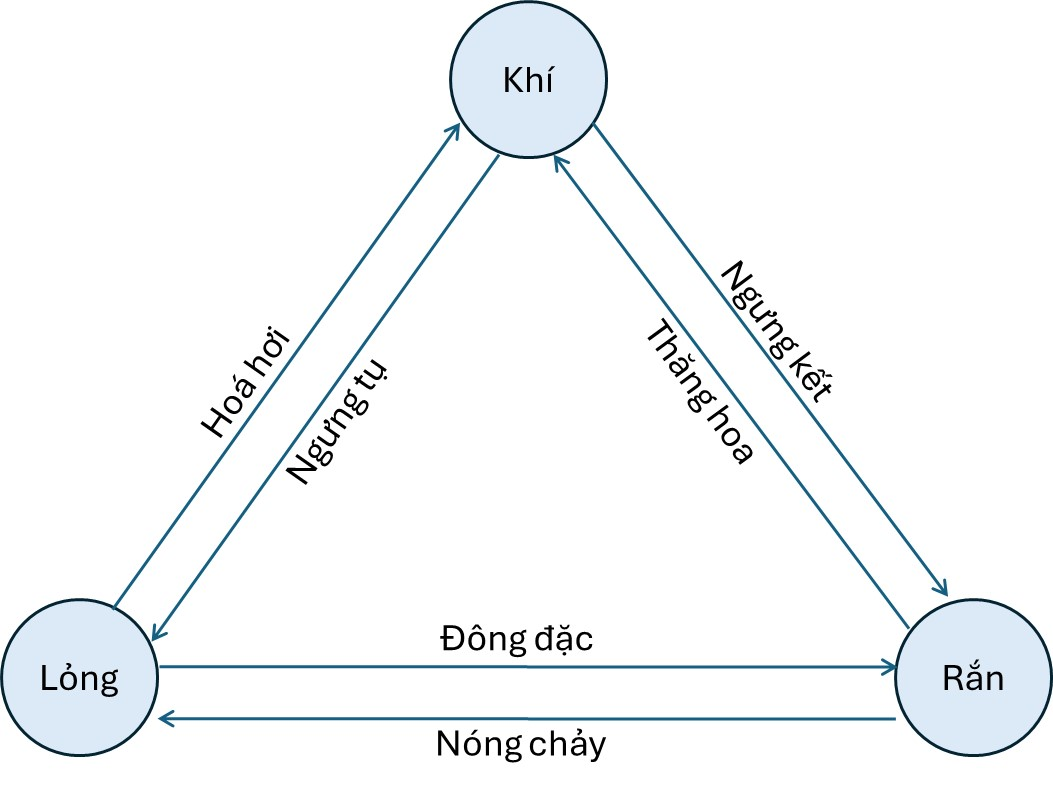
\includegraphics[width=0.5\linewidth]{../figs/VN12-Y24-PH-SYL-001-4}
	\captionof{figure}{Sơ đồ các hình thức chuyển thể.}
\end{center}
\subsection{Sự nóng chảy}
Khi đun nóng đến một nhiệt độ nào đó, vật rắn bắt đầu chuyển trạng thái từ rắn sang lỏng (sự nóng chảy). Chất rắn kết tinh có nhiệt độ nóng chảy xác định (ở một áp suất cụ thể). Chất rắn vô định hình không có nhiệt độ nóng chảy xác định.\\
\textbf{\textit{Ví dụ:}}
\begin{itemize}
	\item Khi nung nóng nước đá ở áp suất tiêu chuẩn, nhiệt độ nước đá tăng dần. Khi đạt đến $\SI{0}{\celsius}$, nước đá bắt đầu tan và trong suốt quá trình hoá lỏng nhiệt độ của nước đá không đổi. Nước đá là chất rắn kết tinh.
	\item Khi nung nóng thỏi sôcôla, thỏi sôcôla mềm đi và chuyển dần sang thể lỏng, trong quá trình này nhiệt độ của thỏi sôcôla vẫn tăng liên tục. Thỏi sôcôla là chất rắn vô định hình.
\end{itemize}
\begin{center}
	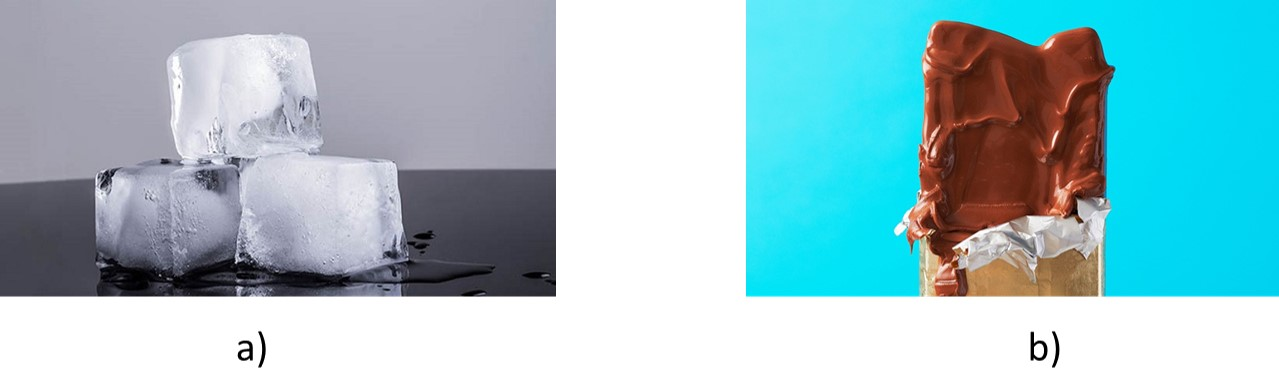
\includegraphics[width=0.6\linewidth]{../figs/VN12-Y24-PH-SYL-001-5}
	\captionof{figure}{a) Nước đá đang tan; b) Thanh sôcôla đang nóng chảy.}
\end{center}
\subsection{Sự hoá hơi}
\subsubsection{Sự bay hơi}
Sự bay hơi là sự hoá hơi xảy ra \textbf{trên bề mặt chất lỏng}. Sự bay hơi xảy ra ở \textbf{nhiệt độ bất kì}.\\
Tốc độ bay hơi của chất lỏng càng nhanh nếu diện tích mặt thoáng càng lớn, tốc độ gió càng lớn, nhiệt độ càng cao, và độ ẩm không khí càng thấp.
\subsubsection{Sự sôi}
Sự sôi là sự hoá hơi xảy ra \textbf{bên trong và trên bề mặt chất lỏng}. Sự sôi xảy ra ở \textbf{nhiệt độ sôi}.\\
Nhiệt độ sôi của chất lỏng phụ thuộc áp suất khí trên mặt thoáng và bản chất của chất lỏng. Trong suốt thời gian sôi, nhiệt độ của chất lỏng không thay đổi.
\begin{center}
	
	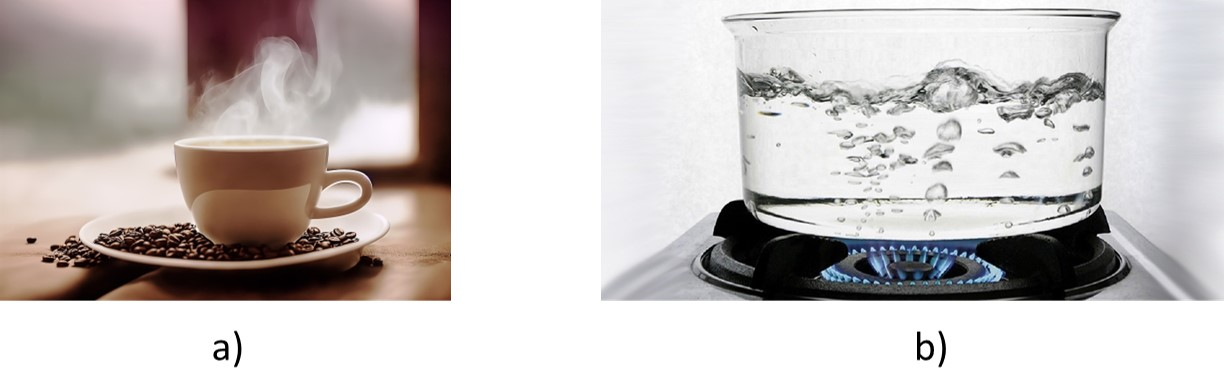
\includegraphics[width=0.65\linewidth]{../figs/VN12-Y24-PH-SYL-001-6}
	\captionof{figure}{a) Nước bay hơi trên mặt thoáng của tách cà phê; b) Nước đang sôi.}
\end{center}
\section{Mục tiêu bài học - Ví dụ minh hoạ}
\begin{dang}{Sử dụng mô hình động học phân tử, nêu được sơ lược cấu trúc của chất rắn, chất lỏng, chất khí.}
	\viduii{2}
	{Năm 1827, khi làm thí nghiệm quan sát các hạt phấn hoa rất nhỏ trong nước bằng kính hiển vi, Brown thấy chúng chuyển động hỗn loạn, không ngừng. Chuyển động này được gọi là chuyển động Brown.\\
		\begin{center}
			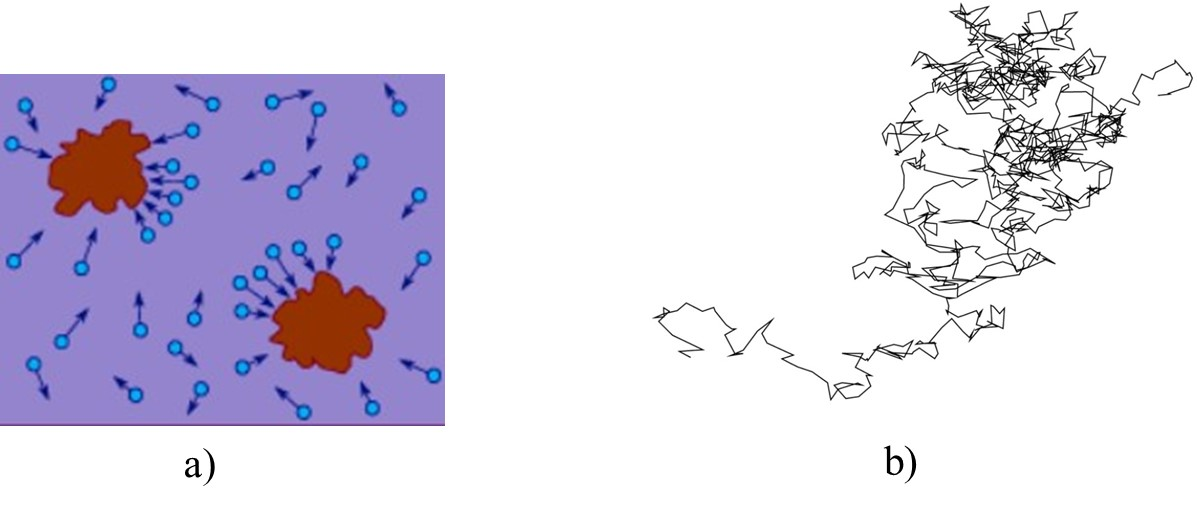
\includegraphics[width=0.6\linewidth]{../figs/VN12-Y24-PH-SYL-001-1}
			\captionof{figure}{a) Mô phỏng sự va chạm giữa các phân tử nước với các hạt phấn hoa; b) Quỹ đạo chuyển động của hạt phấn hoa.}
		\end{center}
		\begin{enumerate}[label=\alph*)]
			\item Tại sao thí nghiệm của Brown được gọi là một trong những thí nghiệm chứng tỏ các phân tử chuyển động hỗn loạn không ngừng?
			\item Làm thế nào để với thí nghiệm của Brown có thể chứng tỏ được khi nhiệt độ của nước càng cao thì các phân tử nước chuyển động càng nhanh?
		\end{enumerate}
		
	}
	{
		\begin{enumerate}[label=\alph*)]
			\item Thông qua việc quan sát hạt phấn hoa trong nước, Brown nhận thấy rằng các hạt phấn hoa lắc lư không ngừng và quỹ đạo chuyển động của hạt phấn hoa hỗn loạn. Mà chuyển động của hạt phấn hoa là do sự va chạm  giữa các phân tử nước với hạt phấn hoa gây ra. Điều này chứng tỏ rằng chuyển động của các phân tử nước cũng hỗn loạn, không ngừng.
			\item Để với thí nghiệm của Brown có thể chứng tỏ được khi nhiệt độ của nước càng cao thì các phân tử nước chuyển động càng nhanh thì chúng ta có thể đun nóng nước rồi quan sát sự thay đổi tốc độ chuyển động của hạt phấn hoa.
		\end{enumerate}
	}
	
	\viduii{2}
	{Hãy giải thích đặc điểm sau đây của thể khí, thể rắn, thể lỏng.
		\begin{enumerate}[label=\alph*)]
			\item Chất khí không có hình dạng và thể tích riêng, luôn chiếm toàn bộ thể tích bình chứa và có thể nén được dễ dàng.
			\item Vật ở thể rắn có thể tích và hình dạng riêng, rất khó nén.
			\item Vật ở thể lỏng có thể tích riêng nhưng không có hình dạng riêng.
		\end{enumerate}
	}
	{
		\begin{enumerate}[label=\alph*)]
			\item Ở thể khí, các phân tử ở xa nhau (khoảng cách giữa các phân tử lớn gấp hàng chục lần kích thước phân tử). Lực tương tác giữa các phân tử rất yếu (trừ trường hợp chúng va chạm nhau) nên các phân tử chuyển động hoàn toàn hỗn loạn. Do đó, khối chất khí không có hình dạng và thể tích riêng mà có hình dạng và thể tích của bình chứa nó.
			\item Ở thể rắn, các phân tử rất gần nhau (khoảng cách giữa các phân tử cỡ kích thước phân tử) và các phân tử sắp xếp có trật tự, chặt chẽ. Lực tương tác giữa các phân tử rất mạnh, giữ cho chúng không di chuyển tự do mà chỉ có thể dao động quanh vị trí cân bằng xác định. Do đó, vật rắn luôn có thể tích và hình dạng riêng xác định, đồng thời rất khó nén.
			\item Khoảng cách giữa các phân tử trong chất lỏng lớn hơn khoảng cách giữa các phân tử trong chất rắn và nhỏ hơn khoảng cách giữa các phân tử trong chất khí. Lực tương tác giữa các phân tử ở thể lỏng lớn hơn lực tương tác giữa các phân tử ở thể khí nên giữ các phân tử không bị phân tán ra xa nhau, do đó chất lỏng có thể tích riêng xác định. Lực tương tác này chưa đủ lớn như trong thể rắn nên các phân tử ở thể lỏng cũng dao động quanh vị trí cân bằng nhưng các vị trí cân bằng này luôn luôn thay đổi. Do đó, khối chất lỏng không có hình dạng riêng xác định mà có hình dạng của bình chứa nó.
		\end{enumerate}
	}
\end{dang}
\begin{dang}{Giải thích được sơ lược một số hiện tượng vật lí liên quan đến sự chuyển thể: sự nóng chảy, sự hoá hơi.}
	\viduii{3}
	{Vận dụng mô hình động học phân tử, em hãy giải thích nguyên nhân gây ra sự nóng chảy của chất rắn kết tinh.
		
	}
	{
		Ở áp suất không đổi, các phân tử ở thể rắn liên kết chặt chẽ với nhau, chúng dao động quanh các vị trí cân bằng xác định. Khi nung nóng chất rắn kết tinh, các phân tử được cung cấp nhiệt năng làm tốc độ chuyển động nhiệt của nó tăng lên, mức độ trật tự trong cấu trúc của các hạt giảm đi.  Điều này dẫn đến khoảng cách trung bình giữa các phân tử tăng.\\
		Nhiệt độ của vật rắn tăng đến một giá trị nào đó thì một số phân tử thắng được lực liên kết với các phân tử xung quanh và thoát khỏi liên kết với chúng, đó là sự khởi đầu của quá trình nóng chảy. Từ lúc này, vật rắn nhận nhiệt lượng để tiếp tục phá vỡ các liên kết tinh thể. Khi trật tự của tinh thể bị phá vỡ hoàn toàn thì quá trình nóng chảy kết thúc, vật rắn chuyển thành khối chất lỏng.
	}
	
	\viduii{3}
	{Vận dụng mô hình động học phân tử, em hãy giải tích nguyên nhân gây ra sự bay hơi và sự sôi.
		
	}
	{\begin{itemize}
			\item \textbf{Giải thích sự bay hơi:}\\
			Các phân tử ở bề mặt chất lỏng tham gia chuyển động nhiệt, trong đó có những phân tử chuyển động hướng ra ngoài chất lỏng. Đồng thời, các phân tử có thể truyền năng lượng cho nhau thông qua quá trình va chạm. Do đó, một số phân tử ở gần mặt thoáng của chất lỏng có động năng đủ lớn để thắng lực liên kết của các phân tử chất lỏng khác thì thoát được ra khỏi mặt thoáng của chất lỏng trở thành các phân tử ở thể hơi.
			\item \textbf{Giải thích sự sôi:}\\
			Khi chất lỏng đến nhiệt độ sôi, do tiếp tục được cung cấp nhiệt nên các phân tử chất lỏng chuyển động nhiệt mạnh hơn, làm phá vỡ sự liên kết giữa các phân tử chất lỏng với nhau. Khi đó các bọt chứa không khí và hơi nước nổi lên trong lòng nước càng ngày càng nhiều, càng nổi lên trên thể tích các bọt khí này càng tăng, tới mặt thoáng thì vỡ, không khí và hơi nước thoát ra ngoài khí quyển.
		\end{itemize}
	}
\end{dang}